\documentclass[12pt]{report}
\usepackage[utf8]{inputenc}
\usepackage[vietnamese]{babel}
\usepackage{array}
\usepackage{booktabs}
\usepackage{longtable}
\usepackage{tabularx}
\usepackage{graphicx}
\usepackage{amsmath}
\usepackage{geometry}
\usepackage{makecell}
\usepackage{ltxtable}
\usepackage{enumitem}
% Thiết lập margins cho A4
\geometry{
    a4paper,
    left=2cm,
    right=2cm,
    top=2.5cm,
    bottom=2.5cm
}

% Định nghĩa kiểu cột mới để văn bản wrap tự động
\newcolumntype{L}[1]{>{\raggedright\arraybackslash}p{#1}}
\newcolumntype{C}[1]{>{\centering\arraybackslash}p{#1}}

\begin{document}

% Trang bìa
\begin{titlepage}
    \begin{flushright}
        
\includegraphics[width=4cm]{logo.jpg}
    \end{flushright}

    \vspace*{1cm}
    \begin{center}
        {\bfseries\Large Khoa Công Nghệ Thông Tin}\\[0.5cm]
        Chuyên ngành: {\bfseries Khoa Học Máy Tính}\\[0.5cm]
        Bộ Môn: {\bfseries Thị Giác Máy Tính}\\
        Lớp 67CS2\\[1.5cm]
        {\bfseries\LARGE Báo Cáo Đồ Án}\\[0.8cm]
        {\bfseries\large Chủ Đề: Background Segmentation (Human)}\\[0.5cm]
        Giảng Viên Hướng Dẫn: Ths. Nguyễn Đình Quý\\[1cm]
        {\large\textbf{Nhóm 6:}}\\[0.5cm]
        \begin{tabular}{ll}
            Hoàng Quốc Vũ      & 4005667 \\
            Tôn Văn Dân        & 0113167 \\
            Nguyễn Duy Hiếu    & 0178167 \\
            Bạch Hưng Bảo      & 0016867 \\
        \end{tabular}
    \end{center}
    \vfill
\end{titlepage}


\newpage

\chapter*{Giới Thiệu về Phân Đoạn Nền}
Phân đoạn nền (Background Segmentation) là một nhiệm vụ quan trọng trong lĩnh vực thị giác máy tính (Computer Vision), với mục tiêu chính là tách biệt đối tượng tiền cảnh (foreground) như con người, xe cộ, đồ vật khỏi phần nền phía sau (background) trong ảnh hoặc video. Khác với các bài toán phân đoạn ngữ nghĩa thông thường, phân đoạn nền nhấn mạnh vào việc loại bỏ thông tin không quan trọng để làm nổi bật đối tượng chính, từ đó giúp các hệ thống xử lý ảnh tập trung hiệu quả hơn vào vùng quan trọng.

Trong đề tài này, nhóm đã triển khai một hệ thống phân đoạn nền sử dụng mô hình DeepLabV3+, một mô hình mạng nơ-ron sâu tiên tiến kết hợp giữa kiến trúc Encoder-Decoder và các module trích xuất đặc trưng đa tỉ lệ (ASPP - Atrous Spatial Pyramid Pooling). Mô hình sử dụng ResNet50 làm backbone nhằm tận dụng khả năng trích xuất đặc trưng mạnh mẽ, giúp cải thiện độ chính xác trong các bối cảnh phức tạp như nền đa dạng, ánh sáng không đồng đều hoặc hình ảnh bị nhiễu.

Thông qua quá trình huấn luyện, mô hình DeepLabV3+ với ResNet50 đã cho kết quả tốt, với chỉ số mIoU đạt trên 96\% trên tập huấn luyện và khoảng 93\% trên tập kiểm tra, thể hiện khả năng học đặc trưng và phân đoạn nền hiệu quả, phù hợp với các ứng dụng thực tế.

\section*{1.2 Đặt vấn đề}
Bài toán phân đoạn nền tuy phổ biến nhưng vẫn gặp nhiều thách thức thực tế:

- Chất lượng ảnh đầu vào thấp hoặc nhiễu ảnh khiến mô hình khó phân biệt được foreground và background.
- Yêu cầu tốc độ xử lý cao trong các ứng dụng thời gian thực như AR, camera giám sát, đòi hỏi mô hình vừa nhanh vừa chính xác.
- Độ phức tạp của nền: các họa tiết hoặc vật thể trong nền có thể gây nhầm lẫn với đối tượng chính.
- Điều kiện ánh sáng thay đổi, góc chụp nghiêng có thể làm sai lệch hình dạng và màu sắc của đối tượng.
- Kích thước và hình dạng đa dạng của đối tượng yêu cầu mô hình phải linh hoạt và tổng quát tốt.
- Độ phân giải ảnh thấp dẫn đến mất chi tiết biên, gây khó khăn cho việc phân đoạn chính xác.

Chính vì những khó khăn trên, việc áp dụng các mô hình học sâu như DeepLabV3+ có khả năng học được các đặc trưng sâu và trừu tượng là cần thiết. Dự án này hướng tới mục tiêu tách phần nền và phần tiền cảnh trong ảnh sao cho hệ thống có thể tập trung vào vùng chứa thông tin quan trọng, từ đó nâng cao chất lượng các bước xử lý phía sau như nhận diện, theo dõi, hoặc chỉnh sửa ảnh.

\section*{Ứng dụng}
Một hệ thống phân đoạn nền hiệu quả có thể mang lại nhiều lợi ích thiết thực:
- Tách rõ vùng đối tượng và nền: xác định chính xác đâu là vật thể chính (con người, vật dụng...) và đâu là nền, làm nền tảng cho nhiều bài toán xử lý ảnh cao hơn.
- Tiền xử lý cho các hệ thống khác: như nhận diện hành động, phân loại ảnh, nhận dạng khuôn mặt, theo dõi đối tượng (object tracking).
- Xóa bỏ thông tin nền không cần thiết: giúp mô hình học sâu tập trung hơn vào vùng quan trọng, giảm nhiễu và tăng hiệu quả học.
- Chỉnh sửa ảnh/video: như xóa phông, thay nền, làm mờ nền, đặc biệt hữu ích trong nhiếp ảnh, thiết kế đồ họa và truyền thông.
- Ứng dụng thời gian thực: như camera an ninh thông minh, AR/VR, hội nghị trực tuyến (Zoom, Google Meet...), nơi cần tách người khỏi nền nhanh và chính xác.

\section*{1.4. Các Nghiên Cứu Liên Quan}
Các nghiên cứu nổi bật liên quan đến phân đoạn nền và các mô hình tương tự:
- Chen et al. (2018) giới thiệu DeepLabV3+, cải tiến phân đoạn ngữ nghĩa với Encoder-Decoder, đạt IoU 89\% trên Cityscapes.
- He et al. (2015) phát triển ResNet, giải quyết vanishing gradient, trở thành backbone phổ biến.
- Ronneberger et al. (2015) đề xuất U-Net, tối ưu cho phân đoạn y tế với skip connections.
- Long et al. (2015) phát triển FCN, đặt nền móng cho phân đoạn pixel-wise.

\section*{Đóng Góp vào Đề Tài}
Phát triển mô hình DeepLabV3+ sử dụng ResNet50: triển khai cụ thể mô hình trong môi trường PyTorch để giải quyết bài toán phân đoạn nền.

Xây dựng pipeline xử lý hoàn chỉnh: từ bước tải và tiền xử lý dữ liệu đến huấn luyện, đánh giá và thử nghiệm mô hình.

Tối ưu hóa hiệu suất và độ chính xác: cải thiện loss và tăng mIoU qua từng epoch, kết quả đạt trên 96\% mIoU ở tập huấn luyện và trên 93\% ở tập kiểm tra.

Ứng dụng kết quả vào thực tế: hệ thống có thể mở rộng để dùng cho AR, chỉnh sửa ảnh, xóa nền trong hội họp online hoặc hỗ trợ các bài toán thị giác máy tính khác.

Phân tích ảnh hưởng điều kiện môi trường: thử nghiệm mô hình trong điều kiện nền phức tạp, ánh sáng không đồng đều, chứng minh khả năng tổng quát của mô hình.

\chapter*{Lý Thuyết Nền Tảng}
\section*{Giới Thiệu về ResNet50}
ResNet50, một biến thể của Residual Network do Microsoft Research giới thiệu năm 2015, gồm 50 lớp và sử dụng Residual Connections để khắc phục vanishing gradient trong mạng sâu. Kiến trúc bao gồm 4 khối residual với các đặc điểm:

- Residual Connections truyền thông tin hiệu quả, giảm mất mát dữ liệu.
- khối (Stage 2-5) với Conv 7x7, BatchNorm, ReLU, và Identity Blocks.
- Sử dụng kernel 3x3 và 1x1, tối ưu hóa tính toán.
- Tích hợp Atrous Convolution trong DeepLabV3+ để mở rộng receptive field.

ResNet50 đóng vai trò backbone, trích xuất đặc trưng cấp thấp (128x128) và cấp cao (32x32x1024) cho phân đoạn nền.

Các đặc điểm chính ResNet50:
- Sử dụng Residual Connections (Kết nối tắt): Cho phép truyền thông tin hiệu quả hơn giữa các lớp, giúp tránh mất mát thông tin khi mạng trở nên sâu hơn.
- Hỗ trợ lan truyền gradient dễ dàng hơn, giúp giảm thiểu vấn đề gradient biến mất trong quá trình huấn luyện mô hình sâu.
- Cải thiện khả năng học của mô hình mà không làm tăng đáng kể số lượng tham số, giữ được hiệu suất cao mà không gây quá tải tính toán.

Kiến trúc 50 lớp với 4 khối residual chính:
- Mạng bao gồm 4 khối residual (Residual Blocks), mỗi khối có 3 lớp convolution.
- Các lớp trong mỗi khối residual bao gồm Batch Normalization và ReLU Activation giúp tăng tính ổn định trong quá trình huấn luyện, giảm hiện tượng overfitting.
- Sử dụng các kernel có kích thước nhỏ (3x3 và 1x1) để tối ưu hóa hiệu suất tính toán, giúp mô hình hoạt động nhanh hơn nhưng vẫn giữ được độ chi tiết của ảnh.

Khả năng mở rộng receptive field với Atrous Convolution:

Khi tích hợp vào DeepLabV3+, ResNet-50 có thể sử dụng Atrous Convolution để tăng receptive field mà không làm tăng số tham số.

Điều này giúp mô hình có thể thu thập thông tin từ một vùng không gian rộng hơn, hỗ trợ tốt hơn cho các bài toán segmentation yêu cầu độ chính xác cao.

Xây dựng mạng ResNet50:

\begin{figure}[h]
    \centering
    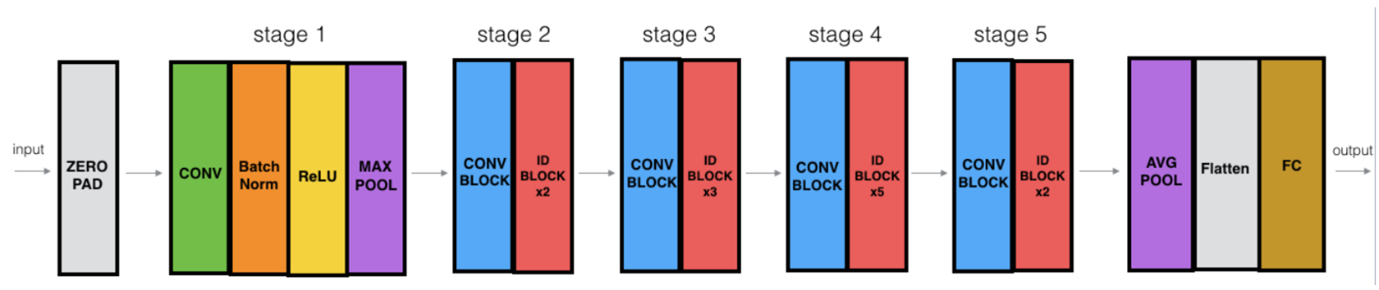
\includegraphics[width=0.8\textwidth]{resnet50.png}
    \caption{Kiến trúc mạng ResNet50}
\end{figure}

"ID BLOCK" trong hình trên là viết tắt của từ Identity block và ID BLOCK x3 nghĩa là có 3 khối Identity block chồng lên nhau. Nội dung hình trên như sau:

- Zero-padding : Input với (3,3)
- Stage 1 : Tích chập (Conv1) với 64 filters với shape(7,7), sử dụng stride (2,2). BatchNorm, MaxPooling (3,3).
- Stage 2 : Convolutiontal block sử dụng 3 filter với size 64x64x256, f=3, s=1. Có 2 Identity blocks với filter size 64x64x256, f=3.
- Stage 3 : Convolutional sử dụng 3 filter size 128x128x512, f=3,s=2. Có 3 Identity blocks với filter size 128x128x512, f=3.
- Stage 4 : Convolutional sử dụng 3 filter size 256x256x1024, f=3,s=2. Có 5 Identity blocks với filter size 256x256x1024, f=3.
- Stage 5 :Convolutional sử dụng 3 filter size 512x512x2048, f=3,s=2. Có 2 Identity blocks với filter size 512x512x2048, f=3.
- The 2D Average Pooling : sử dụng với kích thước (2,2).
- The Flatten.
- Fully Connected (Dense) : sử dụng softmax activation.

\section*{Giới thiệu ASPP}

ASPP giúp mở rộng trường nhìn mà không làm mất độ phân giải không gian. Nó bao gồm:

\begin{figure}[h]
    \centering
    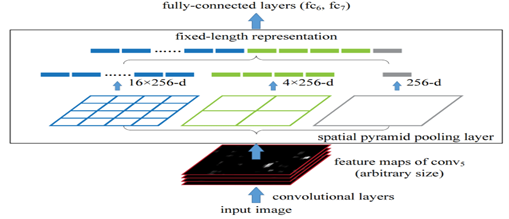
\includegraphics[width=0.8\textwidth]{aspp.png}
    \caption{Spatial Pyramid Pooling (SPP) – Kỹ thuật quan trọng xử lý đầu vào có kích thước thay đổi}
\end{figure}

\begin{itemize}
    \item 1x1 Convolution + Batch Normalization + ReLU.
    \item 3x3 Atrous Convolutions với các tỷ lệ khác nhau (rate = 6, 12, 18) để thu thập thông tin ngữ cảnh ở nhiều tỷ lệ.
\end{itemize}

\begin{figure}[h]
    \centering
    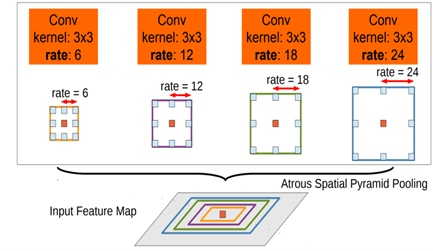
\includegraphics[width=0.9\textwidth]{mau_cam.png}
    \caption{Các nhánh atrous convolution với tỷ lệ khác nhau trong module ASPP (minh họa các trường nhìn khác nhau)}
\end{figure}

\textit{Để phân loại điểm ảnh trung tâm (màu cam), ASPP khai thác các tính năng đa tỷ lệ bằng cách sử dụng nhiều bộ lọc song song với các tỷ lệ khác nhau. Trường nhìn (FOV) hiệu quả được hiển thị bằng các màu khác nhau.}

\begin{itemize}
    \item Image Pooling: Global average pooling giúp nắm bắt thông tin toàn cảnh.
    \item Các đặc trưng từ ASPP được kết hợp lại và truyền qua một lớp 1x1 Convolution + Batch Normalization + ReLU.
\end{itemize}


\section*{Giới Thiệu về DeepLabV3+}

DeepLabV3+, phát triển bởi Google năm 2018, là mô hình phân đoạn ngữ nghĩa cải tiến, kết hợp:
- Encoder: ResNet50 trích xuất đặc trưng, ASPP (Atrous Spatial Pyramid Pooling) với dilation rates 6, 12, 18 thu thập ngữ cảnh đa tỷ lệ.
- Decoder: Kết hợp đặc trưng cấp thấp và ASPP, sử dụng upsampling và Conv 3x3 để phục hồi chi tiết, tạo mặt nạ 512x512x1.

Mô hình này cải thiện ranh giới phân đoạn, phù hợp cho Background Segmentation.

\section*{Cấu trúc và lý thuyết của DeepLab v3+}

DeepLab v3+ là sự kết hợp giữa DeepLab v3 (phiên bản trước đó) và một cấu trúc mã hóa-giải mã (Encoder-Decoder). Dưới đây là các thành phần chính:

\begin{figure}[h]
    \centering
    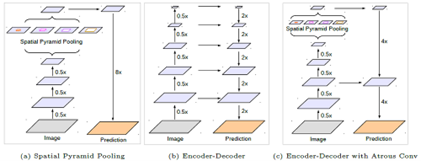
\includegraphics[width=0.8\textwidth]{deeplab-compare.png}
    \caption{a) DeepLabv3 \quad b) Unet \quad c) DeepLabv3+}
\end{figure}

(a) : Các mạng sử dụng mô-đun SPP hoặc ASSP (Atrous Spatial Pyramid Pooling (ASPP), một dạng mở rộng của Spatial Pyramid Pooling (SPP)) ( có thể mã hóa thông tin theo ngữ cảnh đa thang đo bằng cách thăm dò các tính năng đầu vào bằng bộ lọc hoặc hoạt động gộp ở nhiều tốc độ và nhiều FOV (hiệu quả).  
(b) : Với Kiến trúc Encoder-Decoder, thông tin vị trí/không gian được phục hồi. Kiến trúc Encoder-Decoder đã được chứng minh là hữu ích trong các tài liệu như FPN, DSSD, TDM, SharpMask, RED-Net và U-Net cho các mục đích khác nhau.  
(c) : DeepLabv3+ sử dụng (a) và (b). DeepLabv3+ được đề xuất sử dụng những điểm tốt nhất của cả hai thế giới. Với các khối nâng cấp, nối và xử lý trung gian, mô hình có OS=4., mạng lưới nhanh hơn và mạnh hơn đã được phát triển.

DeepLabv3+ mở rộng DeepLabv3 bằng cách thêm một mô-đun giải mã đơn giản nhưng hiệu quả để tinh chỉnh kết quả phân đoạn, đặc biệt là dọc theo ranh giới đối tượng.

\section*{Tích chập Atrous}
Tích chập atrous, còn được gọi là tích chập giãn nở, là một kỹ thuật mạnh mẽ được sử dụng tích cực cho các tác vụ phân đoạn.

Nó cho phép chúng ta kiểm soát độ phân giải mà các tính năng được tính toán bởi DCNN và điều chỉnh FOV của bộ lọc để thu thập thông tin tầm xa.

\begin{figure}[h]
    \centering
    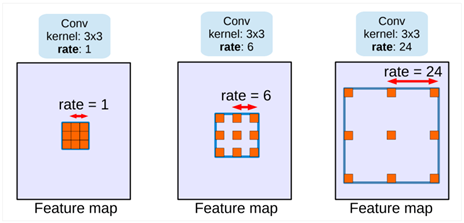
\includegraphics[width=0.8\textwidth]{atrous.png}
    \caption{So sánh tích chập tiêu chuẩn và tích chập atrous}
\end{figure}

Như được chỉ ra trong sơ đồ trên, sự giãn nở của hạt nhân tích chập tương đương với việc chèn các lỗ ('trous' trong tiếng Pháp) giữa các trọng số bộ lọc.

Sử dụng các hạt nhân tích chập giãn nở, người ta có thể dễ dàng sử dụng các mạng được đào tạo trước ImageNet để trích xuất các bản đồ đặc trưng dày đặc hơn. Nó có thể dễ dàng được áp dụng cho một mạng được đào tạo và tích hợp liền mạch trong quá trình đào tạo.

So với phép tích chập thông thường với bộ lọc lớn hơn, phép tích chập atrous cho phép chúng ta mở rộng trường nhìn (FOV) của bộ lọc một cách hiệu quả mà không cần tăng số lượng tham số hoặc lượng tính toán.

\begin{figure}[h]
    \centering
    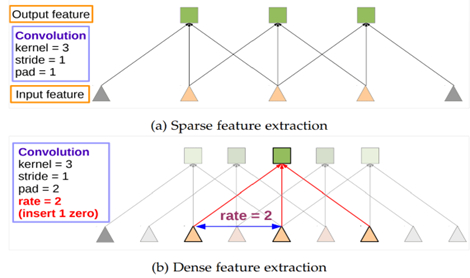
\includegraphics[width=0.8\textwidth]{thua_thot.png}
    \caption{(a) Trích xuất đặc điểm thưa thớt với tích chập tiêu chuẩn trên bản đồ đặc điểm đầu vào có độ phân giải thấp; (b) Trích xuất đặc điểm dày đặc với tích chập atrous với tỷ lệ r=2, được áp dụng trên bản đồ đặc điểm đầu vào có độ phân giải cao.}
\end{figure}

\noindent
a) Trích xuất đặc điểm thưa thớt với tích chập tiêu chuẩn trên bản đồ đặc điểm đầu vào có độ phân giải thấp\\
b) Trích xuất đặc điểm dày đặc với tích chập atrous với tỷ lệ r=2, được áp dụng trên bản đồ đặc điểm đầu vào có độ phân giải cao.


\section*{Kiến trúc của DeepLabV3+}

\begin{figure}[h]
    \centering
    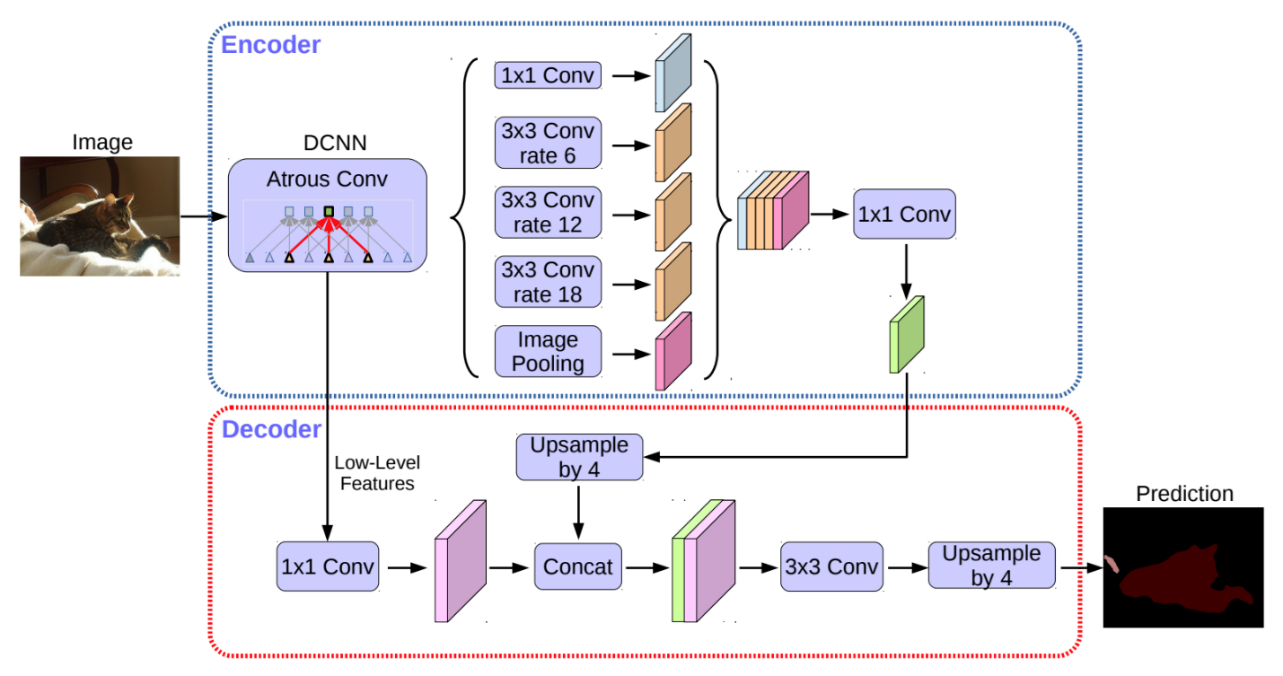
\includegraphics[width=0.8\textwidth]{deeplabv3plus-architecture.png}
    \caption{Kiến trúc chi tiết của DeepLab v3+}
\end{figure}

\textbf{1. Encoder}

Backbone Network:
Phần đầu tiên là một mạng backbone (thường là ResNet hoặc Xception) để trích xuất đặc trưng từ ảnh đầu vào.

Đầu ra của backbone gồm hai phần:
- Đặc trưng sâu (deep features) được truyền qua module ASPP.
- Đặc trưng tầng thấp (low-level features) dùng trong decoder để giúp phục hồi chi tiết không gian.

Atrous Spatial Pyramid Pooling (ASPP):

ASPP giúp mở rộng trường nhìn mà không làm mất độ phân giải không gian. Nó bao gồm:

- 1x1 Convolution + Batch Normalization + ReLU.
- 3x3 Atrous Convolutions với các tỷ lệ khác nhau (rate = 6, 12, 18) để thu thập thông tin ngữ cảnh ở nhiều tỷ lệ.

Để phân loại điểm ảnh trung tâm (màu cam), ASPP khai thác các tính năng đa tỷ lệ bằng cách sử dụng nhiều bộ lọc song song với các tỷ lệ khác nhau. Trường nhìn (FOV) hiệu quả được hiển thị bằng các màu khác nhau.

- Image Pooling: Global average pooling giúp nắm bắt thông tin toàn cảnh.
- Các đặc trưng từ ASPP được kết hợp lại và truyền qua một lớp 1x1 Convolution + Batch Normalization + ReLU.

\textbf{2. Decoder}

Kết hợp đặc trưng tầng thấp và đặc trưng từ ASPP:

- Đặc trưng tầng thấp Ly (có độ phân giải cao hơn) được giảm chiều bằng một lớp 1x1 Convolution + Batch Normalization + ReLU.
- Đặc trưng từ ASPP được upsample (phóng to) lên gấp 4 lần và kết hợp với đặc trưng tầng thấp qua thao tác Concat.

Phục hồi độ phân giải:

- Kết quả kết hợp được truyền qua hai lớp 3x3 Convolution + Batch Normalization + ReLU để tinh chỉnh các đặc trưng.
- Cuối cùng, thực hiện upsample thêm lần nữa (gấp 4 lần) và áp dụng một lớp 1x1 Convolution để tạo ra bản đồ phân đoạn đầu ra.

% Các phần tiếp theo bạn giữ nguyên format như dưới.

\chapter*{Phương pháp đề xuất}
\textbf{Encoder}

3.1.1. DCNN (Deep Convolutional Neural Network): trích xuất đặc trưng
- Sử dụng ResNet50 làm backbone chính với 4 khối chính giúp trích xuất features ở nhiều scale khác nhau. Là bước tiền xử lí đặc trưng cho ảnh đầu vào.
- Cung cấp cả low-level (được lấy sau khối 2) và high-level features

Atrous Spatial Pyramid Pooling (ASPP): Thu thập đặc trưng không gian – ngữ cảnh ở nhiều độ phân giải.
- 5 nhánh song song xử lý đa tỷ lệ
    - Image Pooling: Global context qua AveragePooling2D
    - 1$\times$1 Convolution: Giảm chiều và tích hợp thông tin
    - 3$\times$3 Conv với dilation rate 6
    - 3$\times$3 Conv với dilation rate 12
    - 3$\times$3 Conv với dilation rate 18

3.1.3 Atrous Convolution:
- Mở rộng field of view mà không tăng tham số
- Nắm bắt context ở nhiều tỷ lệ khác nhau
- Dilation rates: 6, 12, 18 cho các vùng nhận thức khác nhau

Feature Fusion:
- Concatenate output từ 5 nhánh ASPP: Các bản đồ đặc trưng từ ASPP được ghép lại theo chiều kênh (depth-wise concatenation). Các bản đồ đặc trưng đầu ra từ các nhánh ASPP có cùng kích thước không gian (H, W). Sắp xếp các nhánh theo thứ tự cố định. Các nhánh có vai trò khác nhau—có nhánh bắt đặc trưng cục bộ, có nhánh bắt đặc trưng toàn cục.

\[
\text{Output} = \text{concat}(F1, F2, F3, F4, F5)
\]

Với:
- F1 là đầu ra từ 1x1 convolution
- F2, F3, F4 là đầu ra từ 3x3 Atrous Convolution với các rate khác nhau
- F5 là đầu ra từ Image Pooling

Sau khi ghép, số lượng kênh của tensor tăng lên 5 lần so với một bản đồ đơn lẻ

Nếu mỗi nhánh có 256 kênh, tổng số kênh sau khi ghép là:
\[
C_{\text{new}} = 256 + 256 + 256 + 256 + 256 = 1280
\]

- Conv 1$\times$1 để tích hợp thông tin: Sau khi ghép xong, ta dùng 1x1 Convolution để giảm số kênh xuống một giá trị hợp lý (thường là 256) trước khi đưa vào Decoder (chỉ thay đổi số kênh, không ảnh hưởng không gian)
\[
W = \text{Ma trận trọng số kích thước } (1280, 256)
\]
Rồi với mỗi vị trí $(x,y)$, ta thực hiện phép nhân ma trận:
\[
F'_{(x,y)} = W^T \cdot F_{(x,y)} + b
\]

- BatchNorm: Ngăn gradient vanishing, cho phép sử dụng learning rate lớn hơn. Đặc biệt quan trọng trong mạng sâu như ResNet50 và ReLU. Giúp model học được các pattern phức tạp. Tính toán đơn giản và hiệu quả. Thêm tính phi tuyến vào mạng. Gradient không bị triệt tiêu với $x > 0$.

\textbf{3.2 Decoder}

3.2.1 Bilinear Upsampling: phương pháp nội suy song tuyến tính dùng để phóng to feature map dùng tính toán toán học giữa các pixel lân cận. Khôi phục kích thước gần như ảnh gốc, giúp kết quả phân vùng bám sát hình dạng thật giúp concat giữa các bước.

Công thức nội suy song tuyến tính:
\[
I_{(x,y)} = \sum_{i=0}^1 \sum_{j=0}^1 w_{ij} \cdot I_{(x_i, y_j)}
\]

Trong đó:
- $I_{(x,y)}$ là giá trị pixel nội suy tại vị trí $(x,y)$
- $I_{(x_i, y_j)}$ là 4 pixel lân cận quanh $(x,y)$
- $w_{ij}$ là hệ số trọng số, phụ thuộc khoảng cách $(x,y)$ và $(x_i, y_j)$

3.2.2 Skip Connection: Lấy feature từ các tầng sớm (thường là sau một vài tầng conv đầu tiên của backbone, như ResNet hoặc Xception) và đưa vào decoder. Những feature sâu thường giàu thông tin ngữ nghĩa nhưng mất chi tiết; các feature cạn thì giữ được chi tiết. Bảo toàn thông tin rìa, kết cấu, hình dạng.

3.2.3 Feature Fusion: Sau khi upsample ASPP output và xử lý low-level feature, concat hai feature maps lại với nhau (trục kênh).

3.2.4 Convolution Refinement: Sau khi concat feature maps, cho qua một chuỗi 3$\times$3 convolution $\rightarrow$ loại bỏ nhiễu, làm rõ thông tin.

\section*{Các API và Công Cụ Sử dụng}

\subsection*{4.1 Framework Deep Learning}
\begin{itemize}
    \item \textbf{PyTorch (1.10+):}
        \begin{itemize}
            \item Framework chính cho việc xây dựng và huấn luyện mô hình
            \item Hỗ trợ tính toán GPU và tối ưu hóa
            \item Ecosystem phong phú và cộng đồng lớn
        \end{itemize}
    \item \textbf{TorchVision:}
        \begin{itemize}
            \item Thư viện hỗ trợ xử lý ảnh và mô hình pre-trained
            \item Cung cấp các transforms chuẩn hóa dữ liệu
            \item Tích hợp sẵn nhiều kiến trúc mạng phổ biến
        \end{itemize}
    \item \textbf{TensorBoard:}
        \begin{itemize}
            \item Công cụ theo dõi và trực quan hóa quá trình huấn luyện
            \item Hiển thị metrics và loss function
            \item So sánh kết quả giữa các thử nghiệm
        \end{itemize}
\end{itemize}

\subsection*{4.2 Thư viện xử lý ảnh}
\begin{itemize}
    \item \textbf{OpenCV:}
        \begin{itemize}
            \item Xử lý ảnh cơ bản và tiền xử lý dữ liệu
            \item Hỗ trợ đọc/ghi nhiều định dạng ảnh
            \item Các phép biến đổi hình học và màu sắc
        \end{itemize}
    \item \textbf{Pillow (PIL):}
        \begin{itemize}
            \item Thao tác với ảnh và augmentation
            \item Tương thích tốt với PyTorch
            \item Xử lý metadata và EXIF
        \end{itemize}
    \item \textbf{Albumentations:}
        \begin{itemize}
            \item Tăng cường dữ liệu nâng cao
            \item Tối ưu hóa cho bài toán phân đoạn
            \item Pipeline linh hoạt và hiệu quả
        \end{itemize}
\end{itemize}

\subsection*{4.3 Công cụ phụ trợ}
\begin{itemize}
    \item \textbf{NumPy:}
        \begin{itemize}
            \item Xử lý dữ liệu số và tính toán ma trận
            \item Tối ưu hóa cho các phép toán đại số tuyến tính
            \item Tích hợp tốt với các thư viện khác
        \end{itemize}
    \item \textbf{Matplotlib:}
        \begin{itemize}
            \item Trực quan hóa kết quả và biểu đồ
            \item Tùy chỉnh linh hoạt và chuyên nghiệp
            \item Hỗ trợ nhiều định dạng xuất
        \end{itemize}
    \item \textbf{tqdm:}
        \begin{itemize}
            \item Hiển thị tiến trình xử lý
            \item Ước tính thời gian hoàn thành
            \item Tích hợp với notebook và CLI
        \end{itemize}
\end{itemize}

\section*{5. Thực nghiệm kiểm tra mô hình}

\subsection*{5.1 Input}
\begin{itemize}
    \item Đưa hình ảnh cần thực hiện semantic segmentation. Mình sẽ đưa ảnh của mình để thực hiện semantic segmentation với size ảnh là 512x512x3.
    \item Chuyển kiểu dữ liệu về float32 để tính toán chính xác, chuẩn hóa giá trị pixel từ [0,255] về [0,1], đảm bảo ảnh có đúng kích thước và formatEncoder.
\end{itemize}

\subsection*{5.2 Encoder}
\begin{itemize}
    \item Tiền xử lí ảnh qua Resnet50: đưa ảnh qua backbone resnet50, giai đoạn đầu giảm kích thước từ 512x512 xuống 256x256 qua conv 7x7. Tiếp tục giảm xuống 128x128 khi qua MaxPooling (bắt đầu trích xuất các đặc trưng cơ bản như cạnh, góc).
    \item Tại 128x128 lưu lại low-level features cho chi tiết cục bộ (dùng ở bước decoder).
    \item Tại 64x64 ảnh được xử lí lấy các pattern phức tạp hơn.
    \item Tại 32$\times$32: Tạo high-level features cho ngữ cảnh toàn cục.
    \item Xử lí qua ASPP: Sau khi ảnh qua bước Resnet50 thì sẽ được đưa ASPP xử lí song song 5 nhánh:
    \begin{itemize}
        \item Image pooling: Nắm bắt context toàn cục của ảnh. Chứa thông tin tổng quan về nội dung ảnh. Giúp model hiểu được bối cảnh tổng thể.
        \item Conv 1x1: Xử lý thông tin tại từng điểm. Giảm chiều và tổng hợp features. Học mối quan hệ tuyến tính giữa các channels.
        \item Atrous Convolution 6, 12, 18: Nắm bắt thông tin ở nhiều mức độ.
    \end{itemize}
    \item Các nhánh này sẽ được ghép lại theo chiều kênh để tổng hợp thông tin tạo ra 1 feature map với ngữ cảnh đầy đủ bao quát, giữ nguyên kích thước không gian (32x32) và tổng hợp channels. Sau đó sẽ được giảm channels qua conv 1x1, giảm độ phức tạp của features, tích hợp thông tin giữa các channels mà vẫn giữ nguyên không gian.
\end{itemize}

\subsection*{5.3 Decoder}
\begin{itemize}
    \item ASPP output sẽ được upsampling lên 4 lần bằng phương pháp bilinear để chuẩn bị cho quá trình fusion với low-level features mà vẫn giữ nguyên các thông tin quan trọng.
    \item Low-level features được lưu lại ở phần trên sẽ được xử lí để phù hợp với ASPP output.
    \item Kết hợp ASPP output với low-level features theo chiều kênh, upsampling lên 4 lần cho bằng với kích thước ban đầu.
\end{itemize}

\subsection*{5.4 Tạo mask cuối cùng}
\begin{itemize}
    \item Chuyển đổi thành probability map.
    \item Mỗi pixel có giá trị từ 0 đến 1.
    \item Thể hiện xác suất pixel thuộc vùng cần segment.
    \item Quá trình này kết hợp cả thông tin ngữ cảnh và chi tiết không gian để tạo ra mask phân đoạn chính xác.
\end{itemize}

\subsection*{Các trường hợp ảnh sau khi qua mô hình}

\begin{table}[h!]
\centering
\renewcommand{\arraystretch}{1.4}
\setlength{\tabcolsep}{2.5pt}
\begin{tabularx}{\textwidth}{|
    >{\centering\arraybackslash}p{1.1cm}|
    >{\centering\arraybackslash}p{2.2cm}|
    >{\centering\arraybackslash}p{3.3cm}|
    >{\centering\arraybackslash}p{2.2cm}|
    >{\centering\arraybackslash}X|}
\hline
\textbf{ID\_picture} & \textbf{Ảnh} & \textbf{Mong Muốn} & \textbf{Kết quả thực tế} & \textbf{Nhận Xét} \\
\hline
P\_1 & Người và nền &
Nền bị xóa tách biệt với người &

\includegraphics[width=1.7cm]{p1_result.png} &
Pass \\
\hline
P\_2 & Người và nền chứa người &
Lấy cả người ở nền &
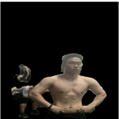
\includegraphics[width=1.7cm]{p2_result.png} &
Pass \\
\hline
P\_3 & Vật thể và nền &
Nền bị xóa tách biệt với vật thể &
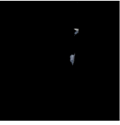
\includegraphics[width=1.7cm]{p3_result.png} &
\makecell{Fail\\Không tách được nền} \\
\hline
P\_4 & Người và vật thể &
Nền bị xóa tách biệt với người ở cạnh vật thể &
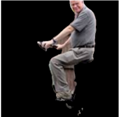
\includegraphics[width=1.7cm]{p4_result.png} &
\makecell{Fail\\Vẫn tách được người\\nhưng vật thể đi cùng thì không} \\
\hline
P\_5 & \makecell{Vật thể\\và nền\\(được làm mờ)} &
Nền bị xóa tách biệt với vật thể &
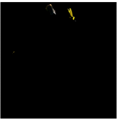
\includegraphics[width=1.7cm]{p5_result.png} &
\makecell{Fail\\Không tách được\\dù nền đã được làm mờ} \\
\hline
\end{tabularx}
\caption{Kết quả kiểm tra phân đoạn nền trên các trường hợp điển hình}
\end{table}

\subsection*{Nhận xét}
\begin{itemize}
    \item Mô hình có thể hoạt động tốt nếu như mục đích chỉ để tách nền với người (ảnh chân dung,...). Còn các trường hợp khác mô hình sẽ hoạt động không đúng hoặc không hoạt động.
    \item Lý do có thể là do dataset chuyên dùng để human\_segmentation. Nếu tổng hợp được dataset lớn hơn thì \% chính xác có thể sẽ cao hơn.
    \item Hoặc cũng có thể mô hình được xây dựng để tách nền với vật thể chứ không phải là phân đoạn ảnh.
\end{itemize}

\section*{Đánh giá hiệu quả mô hình}

Dựa vào các chỉ số train của 5 epoch đầu của U Net và DeepLab V3+:

\begin{table}[h!]
\centering
\renewcommand{\arraystretch}{1.25}
\setlength{\tabcolsep}{4pt}
\begin{tabular}{|p{3.3cm}|p{1.7cm}|p{2.1cm}|p{5.2cm}|}
\hline
\textbf{Chỉ tiêu} & \textbf{U Net} & \textbf{DeepLab V3+} & \textbf{Nhận xét nhanh} \\
\hline
Số epoch đã chạy & 5 & 5 & DeepLab thường cần $\geq$ 20 epoch mới “vọt” mạnh nhờ ASPP; U Net hội tụ rất sớm. \\
\hline
Thời gian/epoch & $\approx$ 4\,300 s & $\approx$ 3\,000 s & U Net mất nhiều VRAM hơn vì giữ full res; DeepLab dùng stride 16 nên nhanh hơn. \\
\hline
Train IoU (cuối) & 0.976 & 0.951 & U Net cao hơn $\approx$ +2,5\%. \\
\hline
Val IoU (cuối) & 0.964 & 0.924 & Khoảng cách $\approx$ +4\%. \\
\hline
Best Val IoU & 0.965 (E4) & 0.924 (E4) & U Net dẫn. \\
\hline
Train Loss (cuối) & 0.0237 & 0.0253 & Tương đương, U Net nhỉnh nhẹ. \\
\hline
Val Loss (cuối) & 0.0357 & 0.0410 & Phù hợp chênh lệch IoU. \\
\hline
Xu hướng loss & Giảm đều, dao động nhẹ (xem hình 1 – trái) & Giảm đều hơn (đường xanh đậm), song cao hơn ban đầu. & -- \\
\hline
Xu hướng IoU & Cao ngay từ đầu, dao động $<$ 1\% (hình 1 – phải) & Tăng ổn định; vẫn còn dư địa nếu train lâu hơn. & -- \\
\hline
Over fit / Under fit & Không rõ rệt: Train IoU – Val IoU $\approx$ +1\% & Chênh $\approx$ +2,7\% $\rightarrow$ chấp nhận được; chưa over fit. & -- \\
\hline
Số tham số $\approx$ & 17 M & 45 M & DeepLab nặng hơn $\times$2,6. \\
\hline
Kích thước receptive field & Hẹp hơn; chủ yếu nhờ skip connection & Rất rộng nhờ Atrous + ASPP $\rightarrow$ lợi thế ảnh cảnh rộng/phức tạp. & -- \\
\hline
\end{tabular}
\caption{Bảng đánh giá hiệu quả mô hình U Net và DeepLabV3+}
\end{table}

\vspace{0.5cm}

\textbf{Hình 1 – Loss \& mIoU}

\begin{itemize}
    \item Train loss (xanh) của DeepLab giảm đều tới $\approx$ 0 .02, val loss (đỏ) tiệm cận $\approx$ 0 .03.
    \item mIoU train $>$ val $\sim$ 0 .03 – 0 .04; không over fit nhưng còn “gap”.
    \item Giảm LR sớm hoặc tăng augmentation có thể thu hẹp gap.
\end{itemize}

\begin{figure}[h]
    \centering
    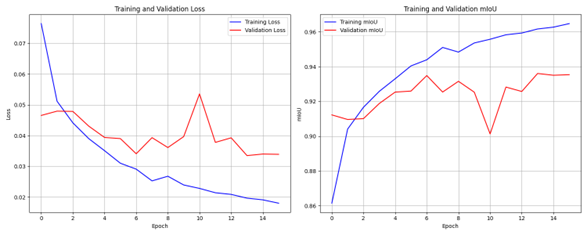
\includegraphics[width=0.8\textwidth]{loss_miou.png}
    \caption{Loss \& mIoU}
\end{figure}

\vspace{0.5cm}

\textbf{Chú thích màu}
\begin{itemize}
    \item Data 1 (nét liền)  $\equiv$ mô hình U Net (cùng tập dữ liệu)
    \item Data (nét đứt) $\equiv$ mô hình DeepLab V3+ (cùng tập)
    \item Trục hoành = Epoch, trục tung = chỉ số tương ứng.
\end{itemize}

\textbf{Hình 2 – 4 biểu đồ}
\begin{figure}[h]
    \centering
    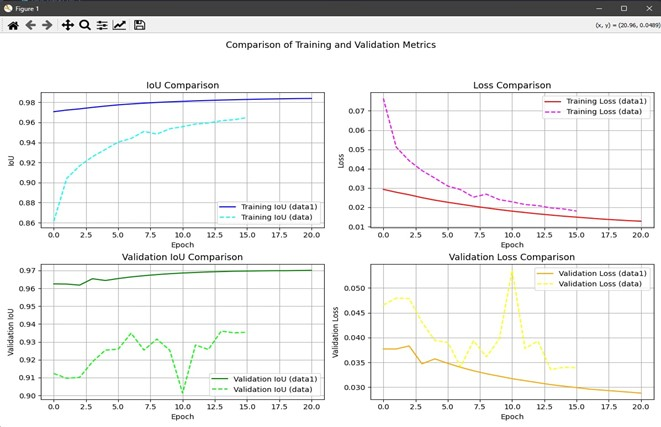
\includegraphics[width=0.8\textwidth]{4_bieudo.jpg}
    \caption{4 biểu đồ Training/Validation IoU, Loss}
\end{figure}

% Bảng 1: Phân tích chi tiết với chiều rộng được tối ưu
\begin{table}[h!]
\renewcommand{\arraystretch}{1.3}
\centering
\footnotesize
\begin{tabularx}{\textwidth}{|L{2.2cm}|L{5.8cm}|L{6.5cm}|}
\hline
\textbf{Biểu đồ} & \textbf{Quan sát chi tiết} & \textbf{Giải thích \& Hệ quả} \\
\hline

Training IoU Comparison &
\begin{itemize}[leftmargin=*,itemsep=1pt,parsep=0pt]
    \item U Net (xanh đậm) khởi động rất cao $\approx$ 0.97, sau $\approx$ 15 epoch tiến sát 0.983 rồi phẳng.
    \item DeepLab (xanh nhạt) bắt đầu thấp $\approx$ 0.86 nhưng leo dốc ổn định, tiệm cận 0.965 lúc epoch 18–20.
    \item Khoảng cách hai đường thu hẹp dần.
\end{itemize}
&
\begin{itemize}[leftmargin=*,itemsep=1pt,parsep=0pt]
    \item U Net học nhanh nhờ skip connection full resolution.
    \item DeepLab cần thời gian để khai thác ASPP + atrous, nhưng vẫn tiến gần.
    \item Không có dấu hiệu overfit ở train IoU (không vượt 0.99).
\end{itemize} \\
\hline

Loss Comparison &
\begin{itemize}[leftmargin=*,itemsep=1pt,parsep=0pt]
    \item Cả hai đường mất mát cùng giảm lũy tiến.
    \item U Net (đỏ) khởi đầu $\approx$ 0.03, xuống dưới 0.015 ở epoch 20.
    \item DeepLab (hồng) cao hơn $\sim$0.05 khi bắt đầu; dốc giảm mạnh trong 10 epoch đầu, sau đó chậm lại và còn $\sim$0.02.
\end{itemize}
&
\begin{itemize}[leftmargin=*,itemsep=1pt,parsep=0pt]
    \item Loss tương quan nghịch với IoU: U Net thấp hơn, phù hợp IoU cao hơn.
    \item Hai đường hội tụ $\Rightarrow$ optimizer, LR schedule phù hợp, không diverge.
\end{itemize} \\
\hline

Validation IoU Comparison &
\begin{itemize}[leftmargin=*,itemsep=1pt,parsep=0pt]
    \item Đường xanh lá đậm (U Net): dao động rất hẹp (0.962$\to$0.971), tăng dần tới gần 0.97.
    \item Xanh lá nhạt (DeepLab): vượt 0.90 ở epoch 1, lên tối đa 0.935$\pm$0.005; có "rãnh" giảm mạnh tại epoch 10 ($\sim$0.90) $\to$ nhiễu dữ liệu / batch đặc thù.
    \item Khoảng cách bền vững $\approx$ 3–4\%.
\end{itemize}
&
\begin{itemize}[leftmargin=*,itemsep=1pt,parsep=0pt]
    \item U Net generalize tốt ngay từ đầu; biên độ dao động $<$0.01 $\rightarrow$ mô hình ổn định.
    \item DeepLab còn "gap" generalization; cần:
    \begin{enumerate}[leftmargin=*,itemsep=1pt,parsep=0pt]
        \item Epoch nhiều hơn,
        \item data augmentation bổ sung,
        \item scheduler giảm LR sau epoch 15.
    \end{enumerate}
\end{itemize} \\
\hline

Validation Loss Comparison &
\begin{itemize}[leftmargin=*,itemsep=1pt,parsep=0pt]
    \item Cam đậm (U Net) giảm mượt từ $\sim$0.037 xuống $\sim$0.029, không tăng đột ngột.
    \item Cam nhạt (DeepLab) dao động 0.033–0.05; spike tại epoch 10 ($>$0.05) cùng chỗ rơi của val IoU $\to$ batch "khó" hoặc LR quá lớn lúc đó.
    \item Sau spike, đường quay lại xu hướng giảm nhưng vẫn cao hơn U Net $\sim$0.003–0.005.
\end{itemize}
&
\begin{itemize}[leftmargin=*,itemsep=1pt,parsep=0pt]
    \item Spike xác nhận điểm nhiễu – khuyến nghị ghi log batch hard case hoặc dùng Gradient Accum/Lookahead.
    \item Khoảng cách loss khớp khoảng cách IoU.
\end{itemize} \\
\hline

\end{tabularx}
\caption{Phán tích chi tiết 4 biểu đồ huấn luyện/đánh giá}
\end{table}

\vspace{1cm}

\textbf{Tổng kết từ 4 biểu đồ:}

% Bảng 2: Sử dụng tabular thông thường vì ít cột hơn
\begin{table}[h!]
\centering
\renewcommand{\arraystretch}{1.4}
\small
\begin{tabular}{|L{3.2cm}|C{3cm}|C{3.2cm}|L{4.8cm}|}
\hline
\textbf{Tiêu chí} & \textbf{U Net (Data 1)} & \textbf{DeepLab V3+ (Data)} & \textbf{Hàm ý} \\
\hline
Tốc độ hội tụ & Rất nhanh – đạt 0.965 val IoU trước epoch 5 & Chậm hơn, nhưng vẫn tăng đều & U Net lợi về thời gian huấn luyện ngắn \\
\hline
Độ ổn định & Đường val IoU \& val loss dao động thấp & Dao động nhiều hơn; spike @ epoch 10 & DeepLab cần regularization / scheduler \\
\hline
Khoảng cách Train–Val & $<$ 1\% (IoU) $\rightarrow$ fit tốt & 2-3\% $\rightarrow$ chưa khai thác hết tiềm năng nhưng chưa overfit & DeepLab tiềm năng cải thiện nếu train dài \\
\hline
Hiệu năng hiện tại (epoch 20) & Val IoU $\approx$ 0.97, Loss $\approx$ 0.029 & Val IoU $\approx$ 0.935, Loss $\approx$ 0.033 & U Net vẫn dẫn đầu $\approx$ +3-3.5\% IoU \\
\hline
\end{tabular}
\caption{So sánh tổng kết mô hình}
\end{table}

\chapter*{7. Tài Liệu Tham Khảo}
\begin{itemize}
    \item \parbox[t]{0.9\textwidth}{Chen, L.-C., et al. ``Encoder-Decoder with Atrous Separable Convolution for Semantic Image Segmentation.'' (2018).}
    \item \parbox[t]{0.9\textwidth}{He, K., et al. ``Deep Residual Learning for Image Recognition.'' (2015).}
    \item \parbox[t]{0.9\textwidth}{Ronneberger, O., et al. ``U-Net: Convolutional Networks for Biomedical Image Segmentation.'' (2015).}
    \item \parbox[t]{0.9\textwidth}{Long, J., et al. ``Fully Convolutional Networks for Semantic Segmentation.'' (2015).}
    \item \parbox[t]{0.9\textwidth}{Sh-tsang. ``Review: DeepLabV3 - Atrous Separable Convolution - Semantic Segmentation.'' Medium.}
    \item \parbox[t]{0.9\textwidth}{LearnOpenCV. ``DeepLabV3+: Ultimate Guide.''}
\end{itemize}

\end{document}
